\section{Testy wydajnościowe i wnioski}

W niniejszym rozdziale zostały zaprezentowane wyniki badań nad efektywnością zaimplementowanego algorytmu. Przedstawiono tutaj zależność czasową między definicją sceny, na podstawie której generowany jest obraz, a zastosowanym podejściem do problemu. Testy były przeprowadzane dla czterech różnych scen (specyficzne ich cechy, jak i ustawienia programu, zostały przedstawione na początku każdego podrozdziału).

\begin{figure}[H]
\centering
  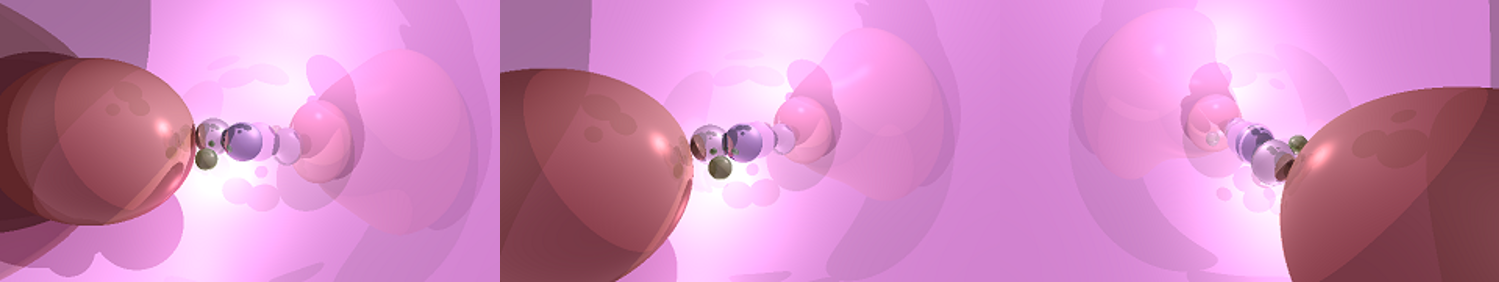
\includegraphics[width=\textwidth]{spheres.png}
    \caption{Spheres}
\end{figure}

Powyższa scena składa się z pięciu sfer o różnych parametrach powierzchniowych - jedna z nich jest półprzezroczysta, inne odbijają światło w podobny sposób jak lustro. Największa z nich otacza pozostałe, dzięki czemu każdy promień wysłany w scenę trafia zawszę w jakąś kulę.

\begin{figure}[H]
\centering
  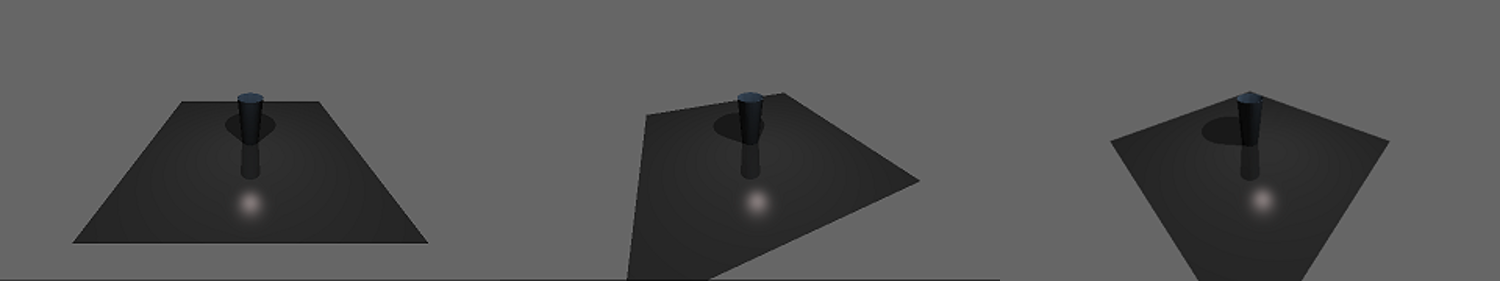
\includegraphics[width=\textwidth]{glass.png}
    \caption{Glass, źródło: }
\end{figure}

Scena autorstwa (!autor!). Składa się ona z 366 trójkątów. Obserwator ustawiony jest pod takim kątem, aby dobrze widzieć całą scenę. Większość promieni pierwotnych nie trafi w żaden obiekt, a szklanka będąca centralną częścią sceny, nie jest przezroczysta (definicje materiałów nie zawierają informacji o przezroczystości).
\pagebreak

\begin{figure}[H]
\centering
  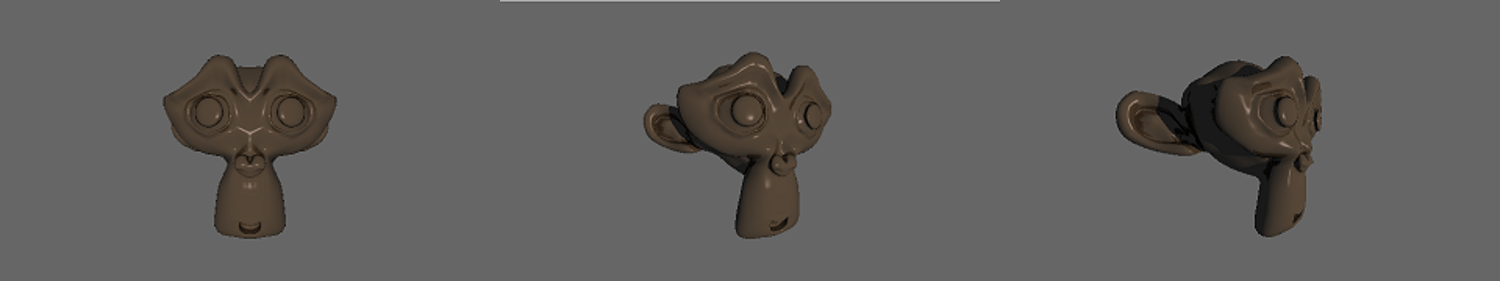
\includegraphics[width=\textwidth]{suzanne.png}
  \caption{Suzanne, źródło: }
\end{figure}


\emph{Suzanne} jest popularnym modelem wykorzystywanym w badaniach dotyczących grafiki komputerowej. Składa się ona z 15488 trójkątów. Definicja materiału została dostarczona przez autorów (MIT) i nie zawiera informacji o przezroczystości. Jak na obiekt takich rozmiarów jest on bardzo skomplikowany.

\begin{figure}[H]
\centering
  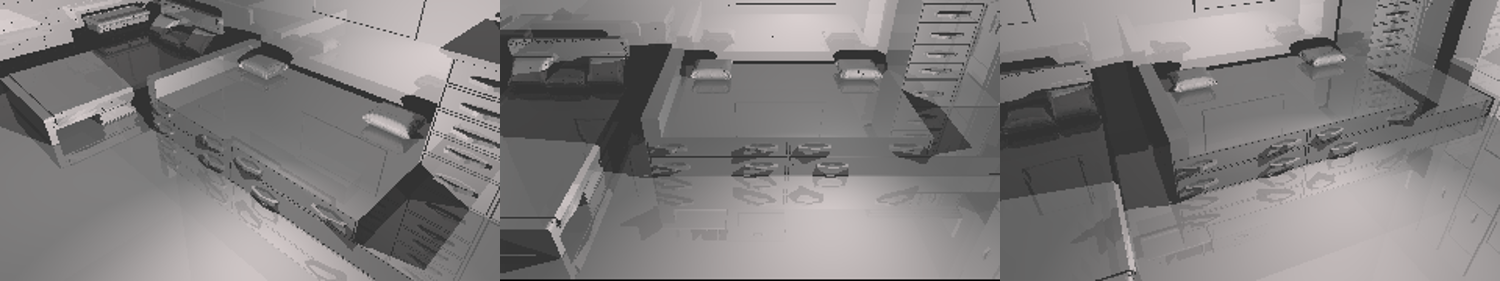
\includegraphics[width=\textwidth]{kid.png}
  \caption{Kid, źródło}
\end{figure}

Scena została pobrana ze strony (strona). Składa się ona z 27946 trójkątów. Autor nie dostarcza definicji materiałów (w założeniu obiekty mają być teksturowane), więc każdy obiekt będzie miał domyślne parametry. To czego nie widać na powyższym obrazku, to brak ściany mającej znajdować się za obserwatorem - w związku z tym większość promieni wtórnych w nic nie trafi.


\subsection{Zależność czasowa od liczby pikseli}

W niniejszym podrozdziale pokazano, w jaki sposób czas generowania obrazu zależy od jego rozmiarów. Testy zostały przeprowadzone dla kilku różnych ujęć scen zaprezentowanych wyżej (kilka takich samych ujęć dla różnej liczby pikseli). Obliczenia dotyczące tego punktu nie zostały zrównoleglone. Parametrom niebędącym przedmiotami tego badania zostały arbitralnie przypisane niniejsze wartości:

\begin{itemize}

\item liczba świateł - 1
\item wyznaczenie cieni - nie
\item głębokość drzewa śledzenia promieni - 3
\item użycie drzewa BSP - nie
\item zrównoleglenie - nie

\end{itemize}

\begin{figure}[!htb]
\advance\leftskip-2cm
\begin{subfigure}{.5\textwidth}
    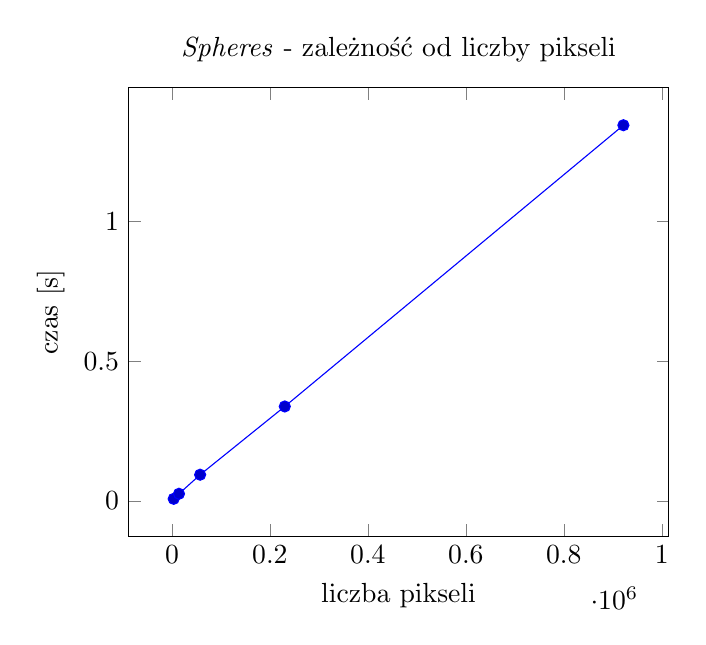
\begin{tikzpicture}
	  \begin{axis}[
	    title=\emph{Spheres} - zależność od liczby pikseli,
	    xlabel=liczba pikseli,
	    ylabel=czas \lbrack s\rbrack,]
	    \addplot coordinates {(3600,0.00764382) (14400,0.0257124) (57600,0.093867) (230400,0.337877) (921600,1.3434)};
	    % if you want the plot to be RED, instead write: \addplot [red,mark=*] coordinates ...
	  \end{axis}
	\end{tikzpicture}
\end{subfigure}
\hspace{2cm}
\begin{subfigure}{.5\textwidth}
		\begin{longtable}{|c|r|} \hline
	    liczba pikseli & \multicolumn{1}{|c|}{spf [s]} \\ \hline
	    3600 (80x45) & 0,008 \\ 
	    14400 (160x90) & 0,026 \\
		57600 (320x180) & 0,094 \\
		230400 (640x360) & 0,338 \\
		921600 (1280x720) & 1,343 \\
		\hline
		\end{longtable}
\end{subfigure}
\end{figure}

\begin{figure}[!htb]
\advance\leftskip-2cm
\begin{subfigure}{.5\textwidth}
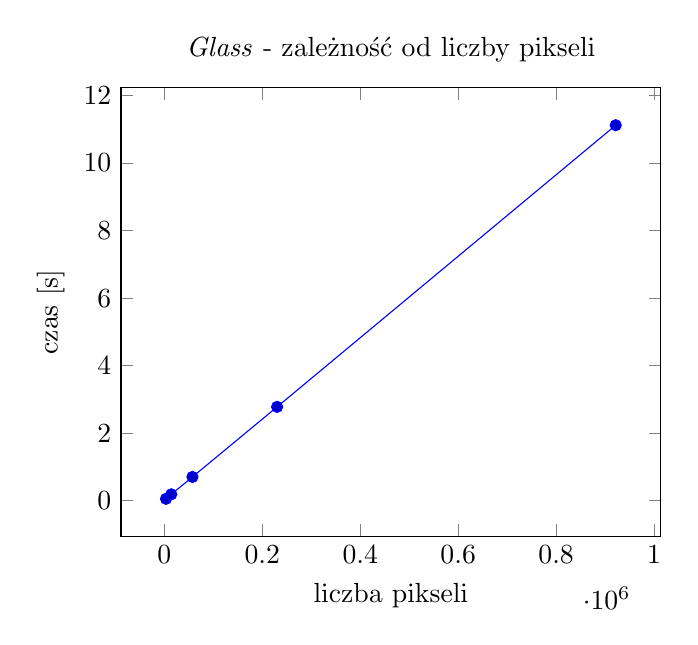
\begin{tikzpicture}
  \begin{axis}[
    title=\emph{Glass} - zależność od liczby pikseli,
    xlabel=liczba pikseli,
    ylabel=czas \lbrack s\rbrack,]
    \addplot coordinates {(3600,0.0567306) (14400,0.191007) (57600,0.705118) (230400,2.77945) (921600,11.1171)};
    % if you want the plot to be RED, instead write: \addplot [red,mark=*] coordinates ...
  \end{axis}
\end{tikzpicture}
\end{subfigure}
\hspace{2cm}
\begin{subfigure}{.5\textwidth}
		\begin{longtable}{|c|r|} \hline
	    liczba pikseli & \multicolumn{1}{|c|}{spf [s]} \\ \hline
	    3600 (80x45) & 0,057 \\ 
	    14400 (160x90) & 0,191 \\
		57600 (320x180) & 0,705 \\
		230400 (640x360) & 2,779 \\
		921600 (1280x720) & 11,117 \\
		\hline
		\end{longtable}
\end{subfigure}
\end{figure}

\begin{figure}[!htb]
\advance\leftskip-2cm
\begin{subfigure}{.5\textwidth}
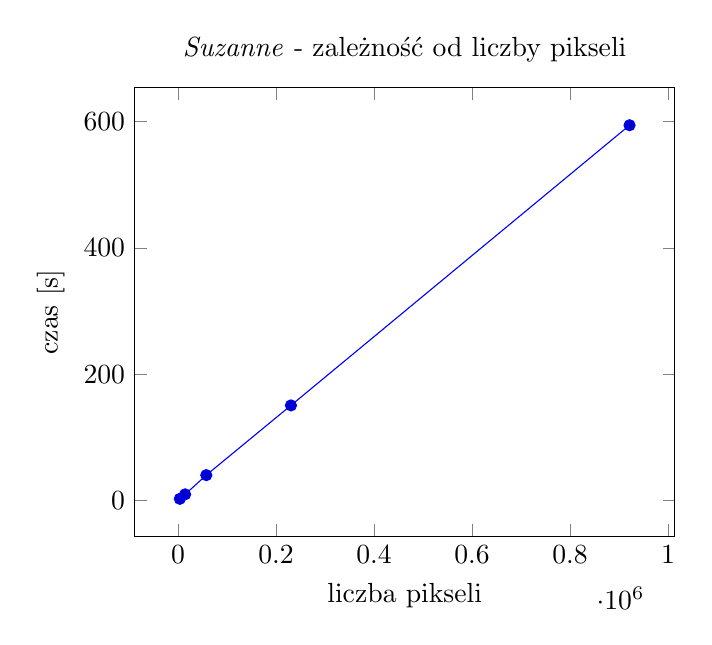
\begin{tikzpicture}
  \begin{axis}[
    title=\emph{Suzanne} - zależność od liczby pikseli,
    xlabel=liczba pikseli,
    ylabel=czas \lbrack s\rbrack,]
    \addplot coordinates {(3600,2.67767) (14400,9.73898) (57600,40.1629) (230400,150.539) (921600,594.091)};
    % if you want the plot to be RED, instead write: \addplot [red,mark=*] coordinates ...
  \end{axis}
\end{tikzpicture}
\end{subfigure}
\hspace{2cm}
\begin{subfigure}{.5\textwidth}
		\begin{longtable}{|c|r|} \hline
	    liczba pikseli & \multicolumn{1}{|c|}{spf [s]} \\ \hline
	    3600 (80x45) & 2,678 \\ 
	    14400 (160x90) & 9,739 \\
		57600 (320x180) & 40,162 \\
		230400 (640x360) & 150,539 \\
		921600 (1280x720) & 594,091 \\
		\hline
		\end{longtable}
\end{subfigure}
\end{figure}


\begin{figure}[!htb]
\advance\leftskip-2cm
\begin{subfigure}{.5\textwidth}
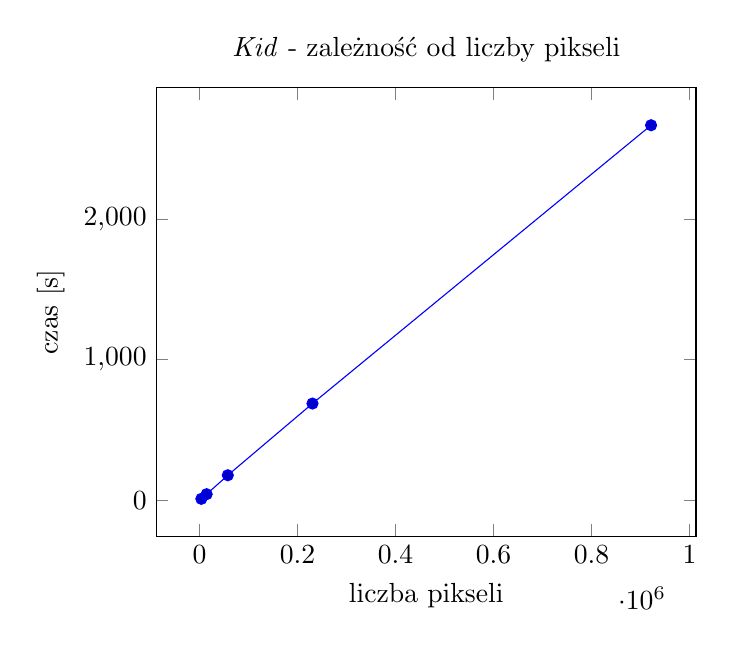
\begin{tikzpicture}
  \begin{axis}[
    title=\emph{Kid} - zależność od liczby pikseli,
    xlabel=liczba pikseli,
    ylabel=czas \lbrack s\rbrack,]
    \addplot coordinates {(3600,11.0737) (14400,44.1641) (57600,178.688) (230400,688.478) (921600,2666.95)};
    % if you want the plot to be RED, instead write: \addplot [red,mark=*] coordinates ...
  \end{axis}
\end{tikzpicture}
\end{subfigure}
\hspace{2cm}
\begin{subfigure}{.5\textwidth}
		\begin{longtable}{|c|r|} \hline
	    liczba pikseli & \multicolumn{1}{|c|}{spf [s]} \\ \hline
	    3600 (80x45) & 11,074 \\ 
	    14400 (160x90) & 44,164 \\
		57600 (320x180) & 178,688 \\
		230400 (640x360) & 688,478 \\
		921600 (1280x720 & 2666,950 \\
		\hline
		\end{longtable}
\end{subfigure}
\end{figure}

Podstawowym wnioskiem, jaki nasuwa się na podstawie otrzymanych wykresów, jest to, że zależność między czasem generowania obrazu a liczbą pikseli jest liniowa, mimo że czas generowania koloru poszczególnych pikseli może być różny. W momencie, w którym promień nie trafi w żaden obiekt, nie zostanie wysłany żaden promień wtórny, co znacząco skraca czas działania algorytmu. Gdy zwiększamy rozmiar obrazu liczba promieni, które trafią w obiekt i takich, które nie trafią nic, rośnie proporcjonalnie do skali powiększenia.

Wiedząc jak zbudowane są sceny, należy zwrócić uwagę na wzrost czasu generowania obrazu w zależności od liczby obiektów. Wykres (!wykres ze stosunkami!) pokazuje, że sceny \emph{Glass} i \emph{Suzzane}, które są podobne do siebie ze względu na budowę (zbudowane są wyłącznie z trójkątów, a generowany obraz jest obrazem zamkniętym - żaden z trójkątów nie wychodzi poza kadr), mają zbliżony stosunek liczby obiektów do czasu generowania klatki. Oznacza to, że ze względu na swoje podobieństwo wzrost liczby obiektów powoduje proporcjonalny wzrost czasu generowania obrazu - jak pokazują pozostałe proste, nie jest to jednak regułą. Dla sceny \emph{Spheres} stosunek liczby obiektów do czasu generowania jest najmniej opłacalny. Jest to spowodowane równomiernym rozrostem drzewa śledzenia promieni - każdy promień trafia w jakiś obiekt, przez co liczba promieni wtórnych rośnie równomiernie. Podobna sytuacja ma miejsce w przypadku sceny \emph{Kid}, jednak tutaj rozrost drzewa jest hamowany przez brak ściany znajdującej się za obserwatorem (część promieni trafia w przestrzeń, co powoduje zmniejszenie liczby promienie wtórnych).

Widzimy, że wzrost czasu generowania obrazu jest w oczywisty sposób zależny od liczby obiektów znajdujących się na scenie, jednak w dużej mierze zależy on również od ich wzajemnego położenia i od położenia obserwatora na scenie (umiejscowienie obserwatora również wpływa na rozrost drzewa, ponieważ to od niego wysyłane są promienie pierwotne). W związku z powyższym przewidzenie ile czasu zajmie generowanie obrazu jest zadaniem trudnym, ale nie niemożliwym - znając wszystkie parametry sceny i algorytmu możemy przewidzieć wersję wydarzeń, w której każdy z promieni napotka na przeszkodę - pesymistyczna złożoność obliczeniowa proponowanego algorytmu (uwzględniającego cienie, dwa rodzaje promieni wtórnych - odbite i załamane) przedstawia się funkcją $T(d,n,o) = (2^d - 1) * o^2 * n$ gdzie:
\\
$d$ - maksymalna głębokość drzewa \\
$o$ - liczba obiektów \\
$n$ - liczba promieni pierwotnych \\ 
\\
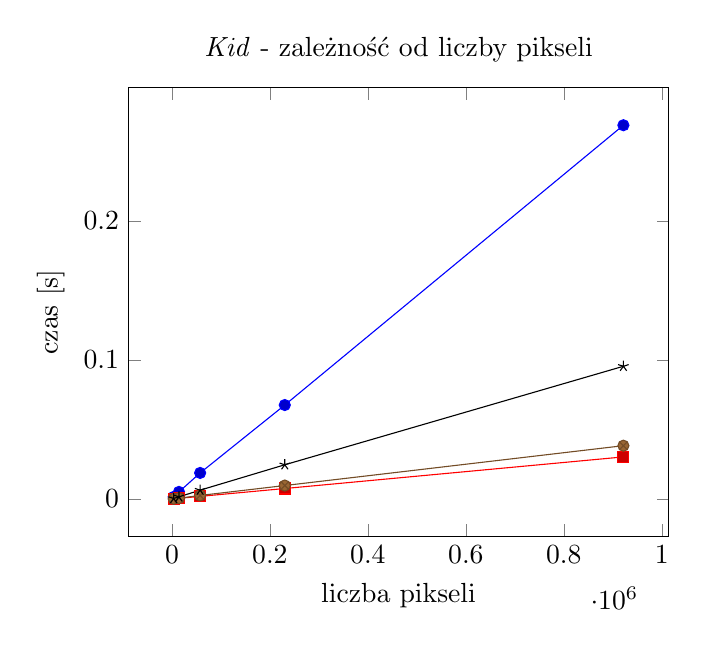
\begin{tikzpicture}
  \begin{axis}[
    title=\emph{Kid} - zależność od liczby pikseli,
    xlabel=liczba pikseli,
    ylabel=czas \lbrack s\rbrack,]
    \addplot coordinates {(3600,0.001528764) (14400,0.00514248) (57600,0.0187734) (230400,0.0675754) (921600,0.26868)};
    \addplot coordinates {(3600,0.000154579) (14400,0.000520455) (57600,0.001921302) (230400,0.007573433) (921600,0.030291826)};
    \addplot coordinates {(3600,0.000172887) (14400,0.000628808) (57600,0.002593162) (230400,0.009719718) (921600,0.038358148)};
    \addplot coordinates {(3600,0.000396253) (14400,0.001580337) (57600,0.006394046) (230400,0.024636012) (921600,0.095432262)};
  \end{axis}
\end{tikzpicture}

\subsection{Zależność czasowa od głębokości drzewa}

W niniejszym podrozdziale zaprezentowano, w jaki sposób zależy czas generowania obrazu od głębokości drzewa śledzenia promieni. Testy zostały przeprowadzone dla kilku różnych ujęć scen zaprezentowanych wyżej (kilka takich samych ujęć dla różnej głębokości drzewa). Obliczenia dotyczące tego punktu nie zostały zrównoleglone. Parametrom niebędącym przedmiotami tego badania zostały arbitralnie przypisane niniejsze wartości:

\begin{itemize}

\item liczba świateł - 1
\item cieniowanie - nie
\item liczba pikseli - 640x360 (230400)
\item użycie drzewa BSP - nie
\item zrównoleglenie - nie

\end{itemize}

\begin{figure}[!htb]
\advance\leftskip-2cm
\begin{subfigure}{.5\textwidth}
\begin{tikzpicture}
  \begin{axis}[
    title=\emph{Spheres} - zależność od głębokości drzewa,
    xlabel=głębokość,
    ylabel=czas \lbrack s\rbrack,]
    \addplot coordinates {(1,0.142384) (2,0.240045) (4,0.444783) (8,0.852983) (16,1.6478)};
    % if you want the plot to be RED, instead write: \addplot [red,mark=*] coordinates ...
  \end{axis}
\end{tikzpicture}
\end{subfigure}
\hspace{2cm}
\begin{subfigure}{.5\textwidth}
		\begin{longtable}{|c|r|} \hline
	    głębokość & \multicolumn{1}{|c|}{spf [s]} \\ \hline
	    1 & 0,142 \\
		2 & 0,240 \\
		4 & 0,445 \\
		8 & 0,853 \\
		16 & 1,648 \\
		\hline
		\end{longtable}
\end{subfigure}
\end{figure}


\begin{figure}[!htb]
\advance\leftskip-2cm
\begin{subfigure}{.5\textwidth}
\begin{tikzpicture}
  \begin{axis}[
    title=\emph{Glass} - zależność od głębokości drzewa,
    xlabel=głębokość,
    ylabel=czas \lbrack s\rbrack,]
    \addplot coordinates {(1,2.16837) (2,2.69988) (4,2.84109) (8,2.86541) (16,2.84629)};
    % if you want the plot to be RED, instead write: \addplot [red,mark=*] coordinates ...
  \end{axis}
\end{tikzpicture}
\end{subfigure}
\hspace{2cm}
\begin{subfigure}{.5\textwidth}
		\begin{longtable}{|c|r|} \hline
	    głębokość & \multicolumn{1}{|c|}{spf [s]} \\ \hline
		1 & 2,168 \\
		2 & 2,670 \\
		4 & 2,841 \\
		8 & 2,865 \\
		16 & 2,846 \\
		\hline
		\end{longtable}
\end{subfigure}
\end{figure}

\begin{figure}[!htb]
\advance\leftskip-2cm
\begin{subfigure}{.5\textwidth}
\begin{tikzpicture}
  \begin{axis}[
    title=\emph{Suzanne} - zależność od głębokości drzewa,
    xlabel=głębokość,
    ylabel=czas \lbrack s\rbrack,]
    \addplot coordinates {(1,129.559) (2,150.077) (4,149.244) (8,151.812) (16,153.429)};
    % if you want the plot to be RED, instead write: \addplot [red,mark=*] coordinates ...
  \end{axis}
\end{tikzpicture}
\end{subfigure}
\hspace{2cm}
\begin{subfigure}{.5\textwidth}
		\begin{longtable}{|c|r|} \hline
	    głębokość & \multicolumn{1}{|c|}{spf [s]} \\ \hline
		1 & 129,559 \\
		2 & 159,077 \\
		4 & 149,244 \\
		8 & 151,812 \\
		16 & 153,429 \\
		\hline
		\end{longtable}
\end{subfigure}
\end{figure}

\begin{figure}[!htb]
\advance\leftskip-2cm
\begin{subfigure}{.5\textwidth}
\begin{tikzpicture}
  \begin{axis}[
    title=\emph{Kid} - zależność od głębokości drzewa,
    xlabel=głębokość,
    ylabel=czas \lbrack s\rbrack,]
    \addplot coordinates {(1,230.193) (2,432.88) (4,843.196) (8,1303.88) (16,1718.51)};
    % if you want the plot to be RED, instead write: \addplot [red,mark=*] coordinates ...
  \end{axis}
\end{tikzpicture}
\end{subfigure}
\hspace{2cm}
\begin{subfigure}{.5\textwidth}
		\begin{longtable}{|c|r|} \hline
	    głębokość & \multicolumn{1}{|c|}{spf [s]} \\ \hline
		1 & 230,193 \\
		2 & 432,880 \\
		4 & 843,196 \\ 
		8 & 1303,880 \\
		16 & 1718,510 \\
		\hline
		\end{longtable}
\end{subfigure}
\end{figure}

Na powyższych wykresach widzimy, że wzrost czasu w zależności od głębokości jest logarytmiczny - jest to spowodowane spadkiem liczby promieni na każdym kolejnym poziomie drzewa (promienie trafiają w próżnię, więc nie są generowane promienie wtórne). Najbardziej wyróżnia się zależność dla sceny \emph{Spheres}, która sprawia wrażenie liniowej. Jest to spowodowane tym, że na tej scenie każdy promień trafia w jakiś obiekt. Teoretycznie funkcje mogłyby rosnąć wykładniczo, ponieważ algorytm dopuszcza generowanie dwóch promieni wtórnych z danego punktu - dzieje się tak, gdy powierzchnia obiektu jest półprzezroczysta - zostaje wysłany promień odbity i promień załamany. W definicji sceny \emph{Spheres} występuje jeden taki obiekt, jednak (jak widać na wykresie) promienie trafiają w niego na tyle rzadko (związane jest to z jego rozmiarami i umiejscowieniem), że nie widzimy tego na wykresie. W przypadku sceny \emph{Kid} każdy obiekt jest w pewnym stopniu przezroczysty, jednak brak ściany pomieszczenia za obserwatorem i tak powoduje spadek promieni wtórnych (jednak jest on wolniejszy niż w przypadku scen \emph{Glass} i \emph{Suzanne}).

\subsection{Zależność czasowa od światła}

W niniejszym podrozdziale zaprezentowano, w jaki sposób zależy czas generowania obrazu od głębokości drzewa śledzenia promieni. Testy zostały przeprowadzone dla kilku różnych ujęć scen zaprezentowanych wyżej, na których losowo rozrzucono zadaną liczbę źródeł światła. Obliczenia dotyczące tego punktu nie zostały zrównoleglone. Parametrom niebędącym przedmiotami tego badania zostały arbitralnie przypisane poniższe wartości:

\begin{itemize}

\item głębokość drzewa śledzenia promieni - 3
\item liczba pikseli - 640x360 (230400)
\item użycie drzewa BSP - nie
\item zrównoleglenie - nie

\end{itemize}

\begin{figure}[!htb]
\advance\leftskip-2cm
\begin{subfigure}{.5\textwidth}
\begin{tikzpicture}
  \begin{axis}[
    title=\emph{Spheres} - zależność od światła,
    xlabel=głębokość,
    ylabel=czas \lbrack s\rbrack,]
    \addplot coordinates {(1,0.251023) (2,0.329837) (4,0.482877) (8,0.786847) (16,1.48653)};
    \addplot coordinates {(1,0.284545) (2,0.318328) (4,0.395992) (8,0.561186) (16,0.561186)};
    % if you want the plot to be RED, instead write: \addplot [red,mark=*] coordinates ...
  \end{axis}
\end{tikzpicture}
\end{subfigure}
\hspace{2cm}
\begin{subfigure}{.5\textwidth}
		\begin{longtable}{|c|r|r|} \hline
		\multirow{2}{*}{liczba świateł} & \multicolumn{2}{|c|}{spf [s]} \\ \cline{2-3}
	    & bez cieni & z cieniami \\ \hline
	    1 & 0,251 & 0,285 \\
	    2 & 0,330 & 0,318 \\
		4 & 0,483 & 0,396 \\
		8 & 0,787 & 0,561 \\
		16 & 1,487 & 1,202 \\
		\hline
		\end{longtable}
\end{subfigure}
\end{figure}


\begin{figure}[!htb]
\advance\leftskip-2cm
\begin{subfigure}{.5\textwidth}
\begin{tikzpicture}
  \begin{axis}[
    title=\emph{Glass} - zależność od światła,
    xlabel=głębokość,
    ylabel=czas \lbrack s\rbrack,]
    \addplot coordinates {(1,2.88157) (2,2.76963) (4,2.78286) (8,2.81478) (16,2.88768)};
    \addplot coordinates {(1,3.27412) (2,3.76403) (4,5.1113) (8,7.44586) (16,10.9446)};
    % if you want the plot to be RED, instead write: \addplot [red,mark=*] coordinates ...
  \end{axis}
\end{tikzpicture}
\end{subfigure}
\hspace{2cm}
\begin{subfigure}{.5\textwidth}
		\begin{longtable}{|c|r|r|} \hline
		\multirow{2}{*}{liczba świateł} & \multicolumn{2}{|c|}{spf [s]} \\ \cline{2-3}
	    & bez cieni & z cieniami \\ \hline
	    1 & 2,881 & 3,274 \\
	    2 & 2,770 & 3,764 \\
		4 & 2,783 & 5,011 \\
		8 & 2,815 & 7,446 \\
		16 & 2,888 & 10,944 \\
		\hline
		\end{longtable}
\end{subfigure}
\end{figure}

\begin{figure}[!htb]
\advance\leftskip-2cm
\begin{subfigure}{.5\textwidth}
\begin{tikzpicture}
  \begin{axis}[
    title=\emph{Suzanne} - zależność od światła,
    xlabel=głębokość,
    ylabel=czas \lbrack s\rbrack,]
    \addplot coordinates {(1,151.408) (2,155.419) (4,162.98) (8,154.59) (16,173.54)};
    \addplot coordinates {(1,146.452) (2,164.65) (4,168.411) (8,201.321) (16,248.212)};
    % if you want the plot to be RED, instead write: \addplot [red,mark=*] coordinates ...
  \end{axis}
\end{tikzpicture}
\end{subfigure}
\hspace{2cm}
\begin{subfigure}{.5\textwidth}
		\begin{longtable}{|c|r|r|} \hline
		\multirow{2}{*}{liczba świateł} & \multicolumn{2}{|c|}{spf [s]} \\ \cline{2-3}
	    & bez cieni & z cieniami \\ \hline
	    1 & 151,408 & 146,452 \\
	    2 & 155,419 & 164,650 \\
		4 & 162,980 & 168,411 \\
		8 & 154,590 & 201,321 \\
		16 & 173,540 & 248,212 \\
		\hline
		\end{longtable}
\end{subfigure}
\end{figure}


\begin{figure}[!htb]
\advance\leftskip-2cm
\begin{subfigure}{.5\textwidth}
\begin{tikzpicture}
  \begin{axis}[
    title=\emph{Kid} - zależność od światła,
    xlabel=głębokość,
    ylabel=czas \lbrack s\rbrack,]
    \addplot coordinates {(1,705.337) (2,716.45) (4,714.296) (8,848.262) (16,853.408)};
    \addplot coordinates {(1,1040.56) (2,1435.52) (4,2330.47) (8,3904.24) (16,6871.04)};
    % if you want the plot to be RED, instead write: \addplot [red,mark=*] coordinates ...
  \end{axis}
\end{tikzpicture}
\end{subfigure}
\hspace{2cm}
\begin{subfigure}{.5\textwidth}
		\begin{longtable}{|c|r|r|} \hline
		\multirow{2}{*}{liczba świateł} & \multicolumn{2}{|c|}{spf [s]} \\ \cline{2-3}
	    & bez cieni & z cieniami \\ \hline
	    1 & 705,337 & 1040,560 \\
	    2 & 716,45 & 1435,520 \\
		4 & 714,296 & 2330,470 \\
		8 & 848,262 & 3904,240 \\
		16 & 853,408 & 6871,040 \\
		\hline
		\end{longtable}
\end{subfigure}
\end{figure}

Z powyższych wykresów wynika, że wpływ liczby źródeł światła na czas generowania obrazu jest znaczny, zwłaszcza w przypadku, w którym śledzimy promień od punktu przecięcia promienia z obiektem do źródła światła (w celu sprawdzenia czy punkt znajduje się w cieniu). Uwzględnienie cieni wymaga przeglądu wszystkich obiektów tak długo, aż nie znajdzie się jakiś między punktem a źródłem światła. W najgorszym przypadku, czyli takim, w którym nic nie rzuca cienia, musimy przejrzeć wszystkie obiekty. W przypadku skomplikowanych scen znacznie wydłuża to czas generowania obrazu (zwłaszcza, że należy to zrobić dla każdego ze źródeł światła - stąd liniowy wzrost czasu generowania obrazu). Wyjątek stanowi scena \emph{Spheres} zawierająca niewielką liczbę obiektów. W sytuacji, w której jakiś obiekt znajduje się w cieniu, nie musimy dla danego punktu wyliczać koloru korzystając z \emph{Modelu Phonha} <!ROZDZIAŁ!> - liczy się tylko światło otoczenia. W związku z tym przy niewielkiej liczbie obiektów koszt jego szukania jest niewielki. Oszczędzamy czas procesora dzięki temu, że nie musimy korzystać ze skomplikowanego modelu światła - paradoksalnie bardziej realistyczny obraz generuje się szybciej.

\subsection{Zależność czasowa od zrównoleglenia}

W niniejszym podrozdziale pokazano, w jakim stopniu zrównoleglenie pozwala na przyspieszenie generowania obrazu. Testy zostały przeprowadzone dla pięciu różnych ziarnistości podziału obrazu (ziarnistość zadania) i dla trzech różnych ilości zaangażowanych procesorów. Testy dla pięciu procesorów zostały przeprowadzone na jednej maszynie, dla dziesięciu na dwóch i dla piętnastu na trzech (wartość podana w tabelach uwzględnia tylko węzły wykonawcze). Każdy z komputerów był maszyną wirtualną, której udostępniono 6 procesorów wirtualnych. Połączenia pomiędzy komputerami były realizowane poprzez technologię \emph{Fast Ethernet}. W dolnej części tabel z wynikami podano ilokrotnie maksymalnie przyspieszyły obliczenia względem podejścia niezrównoleglonego (stosunek czasu obliczeń algorytmu wykonującego się na jednym procesorze do minimalnego czasy otrzymanego w teście). Czas generowania obrazu z wykorzystaniem pojedynczego procesora został wyliczony na nowo i nie ma nic wspólnego z czasami podanymi uprzednio. Powodem takiego podejścia jest to, że testy omówione wyżej były wykonywane na fizycznej maszynie o innej specyfikacji. Parametrom niebędącym przedmiotami tego badania zostały arbitralnie przypisane niniejsze wartości:

\begin{itemize}

\item liczba świateł - 1
\item cieniowanie - tak
\item głębokość drzewa śledzenia promieni - 3
\item użycie drzewa BSP - nie

\end{itemize}

%%%%%%%%%%%%%%%%%%%%%%%%%%%%%%%%%%%%%%%%%%%%%%%%%%%
\begin{figure}[!htb]
\advance\leftskip-2cm
	\begin{subfigure}{.5\textwidth}
	\begin{tikzpicture}
	  \begin{axis}[
	    title=\emph{Spheres} - zależność od zrównoleglenia (640x360),
	    xlabel=głębokość,
	    ylabel=czas \lbrack s\rbrack,]
	    \addplot coordinates {(16,0.179093) (36,0.170406) (64,0.206508) (100,0.213478) (144,0.252288)};
	    \addplot coordinates {(16,0.0881486) (36,0.0854354) (64,0.103843) (100,0.145735) (144,0.218693)};
	    \addplot coordinates {(16,0.0619428) (36,0.063786) (64,0.0976417) (100,0.145701) (144,0.217703)};
	    \addplot coordinates {(16,0.279) (36,0.279) (64,0.279) (100,0.279) (144,0.279)};
	  \end{axis}
	\end{tikzpicture}
	\end{subfigure}
	\hspace{2cm}
	\begin{subfigure}{.5\textwidth}
	\begin{tikzpicture}
	  \begin{axis}[
	    title=\emph{Spheres} - zależność od zrównoleglenia (640x360),
	    xlabel=głębokość,
	    ylabel=czas \lbrack s\rbrack,]
	    \addplot coordinates {(1,0.279) (4,0.170406) (9,0.0854354) (14,0.063786)};
	  \end{axis}
	\end{tikzpicture}
\end{subfigure}
\end{figure}

\begin{figure}[!htb]
\begin{longtable}{|c|r|r|r|} \hline
	    \multirow{2}{*}{liczba fragmentów} & \multicolumn{3}{|c|}{spf [s]} \\ \cline{2-4}
	 	& 4 proc. & 9 proc. & 14 proc. \\ \hline
	    16 & 0,179 & 0,088 & 0,062 \\ 
	    36 & 0,170 & 0,086 & 0,064 \\
		64 & 0,207 & 0,104 & 0,098 \\
		100 & 0,213 & 0,146 & 0,146 \\
		144 & 0,252 & 0,219 & 0,218 \\ \hline
		max przysp. & 1,640 & 3,270 & 4,500 \\
		\hline
\end{longtable}
\end{figure}

%%%%%%%%%%%%%%%%%%%%%%%%%%%%%%%%%%%%%%%%%%%%%%%%%%%%%%%%%%%%%%%%
\begin{figure}[!htb]
\advance\leftskip-2cm
	\begin{subfigure}{.5\textwidth}
	\begin{tikzpicture}
	  \begin{axis}[
	    title=\emph{Glass} - zależność od zrównoleglenia (640x360),
	    xlabel=głębokość,
	    ylabel=czas \lbrack s\rbrack,]
	    \addplot coordinates {(16,1.09964) (36,1.05298) (64,1.03611) (100,1.02236) (144,1.05367)};
	    \addplot coordinates {(16,0.742264) (36,0.548189) (64,0.513832) (100,0.507293) (144,0.544521)};
	    \addplot coordinates {(16,0.479671) (36,0.407425) (64,0.311017) (100,0.322993) (144,0.344262)};
	    \addplot coordinates {(16,2.401) (36,2.401) (64,2.401) (100,2.401) (144,2.401)};
	    % if you want the plot to be RED, instead write: \addplot [red,mark=*] coordinates ...
	  \end{axis}
	\end{tikzpicture}
	\end{subfigure}
		\hspace{2cm}
		\begin{subfigure}{.5\textwidth}
	\begin{tikzpicture}
	  \begin{axis}[
	    title=\emph{Spheres} - zależność od zrównoleglenia (640x360),
	    xlabel=głębokość,
	    ylabel=czas \lbrack s\rbrack,]
	    \addplot coordinates {(1,2.401) (4,1.02236) (9,0.507293) (14,0.311017)};
	  \end{axis}
	\end{tikzpicture}
	\end{subfigure}
\end{figure}

\begin{figure}[!htb]
\begin{longtable}{|c|r|r|r|} \hline
	    \multirow{2}{*}{liczba fragmentów} & \multicolumn{3}{|c|}{spf [s]} \\ \cline{2-4}
	 	& 4 proc. & 9 proc. & 14 proc. \\ \hline
	    16 & 1,100 & 0,742 & 0,480 \\ 
	    36 & 1,053 & 0,548 & 0,407 \\
		64 & 1,036 & 0,514 & 0,311 \\
		100 & 1,022 & 0,507 & 0,323 \\
		144 & 1,053 & 0,545 & 0,344 \\ \hline
		max przysp. & 2,350 & 4,730 & 7,720  \\
		\hline
\end{longtable}
\end{figure}

%%%%%%%%%%%%%%%%%%%%%%%%%%%%%%%%%%%%%%%%%%%%%%%%%%%%%%%%%%%%%%%%
\begin{figure}[!htb]
\advance\leftskip-2cm
	\begin{subfigure}{.5\textwidth}
	\begin{tikzpicture}
	  \begin{axis}[
	    title=\emph{Suzanne} - zależność od zrównoleglenia (640x360),
	    xlabel=głębokość,
	    ylabel=czas \lbrack s\rbrack,]
	    \addplot coordinates {(16,205.605) (36,206.972) (64,209.42) (100,217.794) (144,205.472)};
	    \addplot coordinates {(16,75.4728) (36,70.136) (64,71.2841) (100,70.7879) (144,71.007)};
	    \addplot coordinates {(16,52.8091) (36,37.398) (64,39.9895) (100,37.832) (144,37.0606)};
	    \addplot coordinates {(16,336.1612) (36,336.1612) (64,336.1612) (100,336.1612) (144,336.1612)};
	  \end{axis}
	\end{tikzpicture}
	\end{subfigure}
	\hspace{2cm}
		\begin{subfigure}{.5\textwidth}
	\begin{tikzpicture}
	  \begin{axis}[
	    title=\emph{Spheres} - zależność od zrównoleglenia (640x360),
	    xlabel=głębokość,
	    ylabel=czas \lbrack s\rbrack,]
	    \addplot coordinates {(1,336.1612) (4,205.472) (9,70.136) (14,37.0606)};
	  \end{axis}
	\end{tikzpicture}
	\end{subfigure}
\end{figure}

\begin{figure}[!htb]
\begin{longtable}{|c|r|r|r|} \hline
	    \multirow{2}{*}{liczba fragmentów} & \multicolumn{3}{|c|}{spf [s]} \\ \cline{2-4}
	 	& 4 proc. & 9 proc. & 14 proc. \\ \hline
	    16 & 205,605 & 75,473 & 52,809 \\ 
	    36 & 206,972 & 70,136 & 37,398 \\
		64 & 209,420 & 71,284 & 39,900 \\
		100 & 217,794 & 70,788 & 37,383 \\
		144 & 205,472 & 71,007 & 37,061 \\ \hline
		max przysp. & 1,640 & 4,790 & 9,070 \\
		\hline
\end{longtable}
\end{figure}

%%%%%%%%%%%%%%%%%%%%%%%%%%%%%%%%%%%%%%%%%%%%%%%%%%%%%%%%%%%%%%%%%
\begin{figure}[!htb]
\advance\leftskip-2cm
	\begin{subfigure}{.5\textwidth}
	\begin{tikzpicture}
	  \begin{axis}[
	    title=\emph{Kid} - zależność od zrównoleglenia (640x360),
	    xlabel=głębokość,
	    ylabel=czas \lbrack s\rbrack,]
	    \addplot coordinates {(16,1634.56) (36,1624.21) (64,1616.771) (100,1620.153) (144,1647.817)};
	    \addplot coordinates {(16,647.817) (36,565.67) (64,567.067) (100,563.411) (144,575.474)};
	    \addplot coordinates {(16,439.232) (36,375.321) (64,318.538) (100,311.411) (144,306.143)};
	    \addplot coordinates {(16,2677.71) (36,2677.71) (64,2677.71) (100,2677.71) (144,2677.71)};
	  \end{axis}
	\end{tikzpicture}
	\end{subfigure}
		\hspace{2cm}
	\begin{subfigure}{.5\textwidth}
	\begin{tikzpicture}
	  \begin{axis}[
	    title=\emph{Spheres} - zależność od zrównoleglenia (640x360),
	    xlabel=głębokość,
	    ylabel=czas \lbrack s\rbrack,]
	    \addplot coordinates {(1,2677.71) (4,1616.771) (9,563.411) (14,306.143)};
	  \end{axis}
	\end{tikzpicture}
	\end{subfigure}
\end{figure}
%%%%%%%%%%%%%%%%%%%%%%%%%%%%%%%%%%%%%%%%%%%%%%%%%%%%%%%%%%%%%%%%%%%


\begin{figure}[!htb]
\begin{longtable}{|c|r|r|r|} \hline
	    \multirow{2}{*}{liczba fragmentów} & \multicolumn{3}{|c|}{spf [s]} \\ \cline{2-4}
	 	& 4 proc. & 9 proc. & 14 proc. \\ \hline
	    16 & 1634,560 & 647,817 & 439,232 \\ 
	    36 & 1624,210 & 565,670 & 375,321 \\
		64 & 1616,771 & 567,067 & 318,538 \\
		100 & 1620,153 & 563,411 & 311,411 \\
		144 & 1639,121 & 575,474 & 306,143 \\ \hline
		max przysp. & 1,660 & 4,750 & 8,750  \\
		\hline
\end{longtable}
\end{figure}

Najważniejszym wnioskiem płynącym z powyższych badań jest to, że wraz ze wzrostem liczby węzłów czas generowania maleje logarytmicznie. Oznacza to, że w pewnym momencie zwiększania rozmiarów klastra, nie uzyskamy żadnego przyspieszenia obliczeń. Jest to wniosek zgodny z oczekiwaniami - maksymalna liczba komputerów, której moc obliczeniową można by wykorzystać, nie będzie większa od liczby pikseli obrazu (przynajmniej dla tej metody zrównoleglenia). Górne ograniczenie rozmiarów klastra (dla zadanej wielkości obrazu) jest oczywiście niższe ze względu na czas potrzebny do przesłania informacji pomiędzy węzłami.

Zastanówmy się teraz nad optymalną ziarnistością zadania (liczbą wycinków obrazu). Najciekawiej prezentuje się wykres dotyczący sceny \emph{Spheres} - wraz ze wzrostem liczby wycinków, drastycznie spada wydajność klastra. Dzieje się tak dlatego, ponieważ więcej czasu zajmuje przesyłanie danych pomiędzy węzłami niż rzeczywiste obliczenia. Na pozostałych wykresach liczba wycinków zdaje się nie mieć takiego znaczenia, jednak jest to spowodowane zastosowaną skalą. Wg. danych z tabeli <!numer tabeli!>, optymalną liczba wycinków dla 14 procesów oscyluje wokół wartości 64. Dla pozostałych scen czas generowania klatki spada wraz ze wzrostem ziarnistości. Warto zwrócić uwagę, że dla 14 procesów czas działania algorytmu dla 16 fragmentów jest najdłuższy - jest to spowodowane tym, że po policzeniu pierwszej partii zadań wiele węzłów pozostaje bezczynnych. Dane pokazują również, że optymalna ziarnistość zmienia się wraz ze zmianą rozmiaru klastra.

\subsection{Wykorzystanie drzewa BSP}

W niniejszym podrozdziale pokazano, w jakim stopniu wykorzystanie drzewa BSP pozwala na przyspieszenie generowania obrazu.  W dolnej części tabel z wynikami podano ilokrotnie maksymalnie przyspieszyły obliczenia względem podejścia niezrównoleglonego (stosunek czasu obliczeń algorytmu wykonującego się na jednym procesorze do minimalnego czasy otrzymanego w teście) oraz czas budowy drzewa BSP.
Parametrom niebędącym przedmiotami tego badania zostały arbitralnie przypisane poniższe wartości:

\begin{itemize}

\item głębokość drzewa śledzenia promieni - 3
\item liczba pikseli - 640x360 (230400)
\item użycie drzewa BSP - nie
\item liczba świateł - 1
\item cieniowanie - tak
\item liczba węzłów wykonawczych - 14 

\end{itemize}



\begin{figure}[!htb]
\advance\leftskip-2cm
	\begin{subfigure}{.5\textwidth}
	\begin{tikzpicture}
	  \begin{axis}[
	    title=\emph{Glass} - BSP 0.107058,
	    xlabel=głębokość,
	    ylabel=czas \lbrack s\rbrack,]
	    \addplot coordinates {(16,5.21946) (36,3.8034) (64,3.57917) (100,3.40521) (144,3.53286)};
	    \addplot coordinates {(16,4.99529) (36,2.71377) (64,2.48849) (100,2.2844) (144,2.33781)};
	  \end{axis}
	\end{tikzpicture}
	\end{subfigure}
	\hspace{2cm}
	\begin{subfigure}{.5\textwidth}
	\begin{longtable}{|c|r|r|} \hline
	    \multirow{2}{*}{liczba fragmentów} & \multicolumn{2}{|c|}{spf [s]} \\ \cline{2-3}
	    & brak bryły ot. & z bryłą ot. \\ \hline
	    16 & 5,219 & 4,995 \\ 
	    36 & 3,803 & 2,714 \\
		64 & 3,579 & 2,488 \\
		100 & 3,405 & 2,284 \\
		144 & 3,533 & 2,338 \\ \hline
		max przysp. & 0,700 & 1,050 \\ \hline
		czas gen. drzewa [s] &  \multicolumn{2}{|c|}{0,107} \\ \hline
	\end{longtable}
\end{subfigure}
\end{figure}
\pagebreak
\begin{figure}[!htb]
\advance\leftskip-2cm
	\begin{subfigure}{.5\textwidth}
	\begin{tikzpicture}
	  \begin{axis}[
	    title=\emph{Suzzane} - BSP 317.279,
	    xlabel=głębokość,
	    ylabel=czas \lbrack s\rbrack,]
	    \addplot coordinates {(16,14.3402) (36,10.0665) (64,9.23015) (100,8.29159) (144,8.06655)};
	    \addplot coordinates {(16,16.6061) (36,9.51138) (64,8.03645) (100,7.68939) (144,8.03335)};
	  \end{axis}
	\end{tikzpicture}
	\end{subfigure}
	\hspace{2cm}
	\begin{subfigure}{.5\textwidth}
	\begin{longtable}{|c|r|r|} \hline
	    \multirow{2}{*}{liczba fragmentów} & \multicolumn{2}{|c|}{spf [s]} \\ \cline{2-3}
	    & brak bryły ot. & z bryłą ot. \\ \hline
	    16 & 14,340 & 16,606 \\ 
	    36 & 10,067 & 9,511 \\
		64 & 9,230 & 8,036 \\
		100 & 8,292 & 7,689 \\
		144 & 8,067 & 8,033 \\ \hline
		max przysp. & 41,670 & 43,710 \\ \hline
		czas gen. drzewa [s] &  \multicolumn{2}{|c|}{317,279} \\ \hline
	\end{longtable}
\end{subfigure}
\end{figure}

Metoda śledzenia promieni wykorzystująca drzewo BSP pozwoliła na zmniejszenie czasu generowania obliczeń sceny \emph{Suzanne} do kilku sekund. Początkowy (i co ważne jednorazowy) koszt budowy drzewa przyniósł pożądane rezultaty. Inaczej ma się sytuacja w przypadku sceny \emph{Glass}, która, jak wynika z powyższych danych, jest przypadkiem sceny, dla której korzystanie z drzewa BSP jest nieopłacalne - nie dość, że musieliśmy ponieść koszt związany z jego budową, to jeszcze generowanie kolejnych klatek trwa dłużej niż w przypadku algorytmu niezrównoleglonego. Jakie cechy musi posiadać scena, żeby korzystanie z drzewa BSP było opłacalne i w jaki sposób możemy poprawić jego działanie?

Podstawową problemem sceny \emph{Glass} jest duża liczba promieni pierwotnych, które w nic nie trafiają. Biorąc pod uwagę, że obserwator widzi całą scenę, to większość płaszczyzn dzielących jest przez te promienie przecinane (w zależności od ich nachylenia). W takiej sytuacji algorytm szukania najbliższego obiektu więcej czasu spędza na trawersowaniu drzewa niż miałoby to miejsce w przypadku przeglądu zupełnego - odwiedzi on większość węzłów drzewa. Kolejnym czynnikiem mogącym powodować problem jest wzajemne ułożenie wielokątów na scenie. W sytuacji, w której tworzą one zbiór wypukły, wybieranie płaszczyzny dzielącej spośród tych wyznaczanych przez te wielokąty, sprawia, że żadna z nich nie podzieli przestrzeni. Częściowym rozwiązaniem tego problemu jest szukanie kandydatów na płaszczyzny dzielące nie tylko wśród takich, które pokrywają się w wielokątami sceny, ale też wśród płaszczyzn prostopadłych do tych wieloboków - takie podejście zostało zaimplementowane w testowanym algorytmie.

W celu polepszenia wydajności drzew BSP należy się skupić na czterech elementach: wprowadzeniu brył otaczających (redukcja liczby promieni nietrafiających w żaden obiekt, dla których trzeba by było przeprowadzać testy z wykorzystaniem drzewa BSP), poszukiwaniu lepszej metody wyboru kandydatów na płaszczyzny dzielące, ulepszeniu funkcji oceny płaszczyzny (np. zastosowanie funkcji SAH - !ROZDZIAŁ!), lub poprawie algorytmu trawersowania drzewa.

W celu pokazania, w jakim stopniu wprowadzenie brył otaczających może poprawić rezultaty, testowane sceny zostały zamknięte w prostopadłościanach. Jak widać na wykresie (!wykres szklanka!) zysk czasowy wynikający z zastosowania bryły otaczającej jest znaczący, jednak czas generowania obrazu ciągle jest lepszy dla przeglądu zupełnego. W przypadku \emph{Suzanne} różnica zdaje się być niewielka. Wynika to z położenia obserwatora - w sytuacji, w której znajduje się on blisko obiektu (stosunkowo mało promieni pierwotnych nie trafia w nic), zastosowanie bryły otaczającej w kształcie prostopadłościanu redukuje niewielką liczbę testów. Gdyby obserwator zaczął się oddalać od obiektu, to czas generowania obrazu z wykorzystaniem drzewa BSP by rósł, jednak dzięki wykorzystaniu bryły otaczającej tendencja się odwróci. Niżej przedstawiono mapy cieplne obrazujące które piksele liczyły się najdłużej. Im jaśniejszy obszar tym jego wygenerowanie zajęło więcej czasu. Szum pojawiający się na obrazach jest najprawdopodobniej spowodowany przełączaniem się procesów.

\begin{figure}[h!]
\centering
  \caption{Przegląd zupełny}
  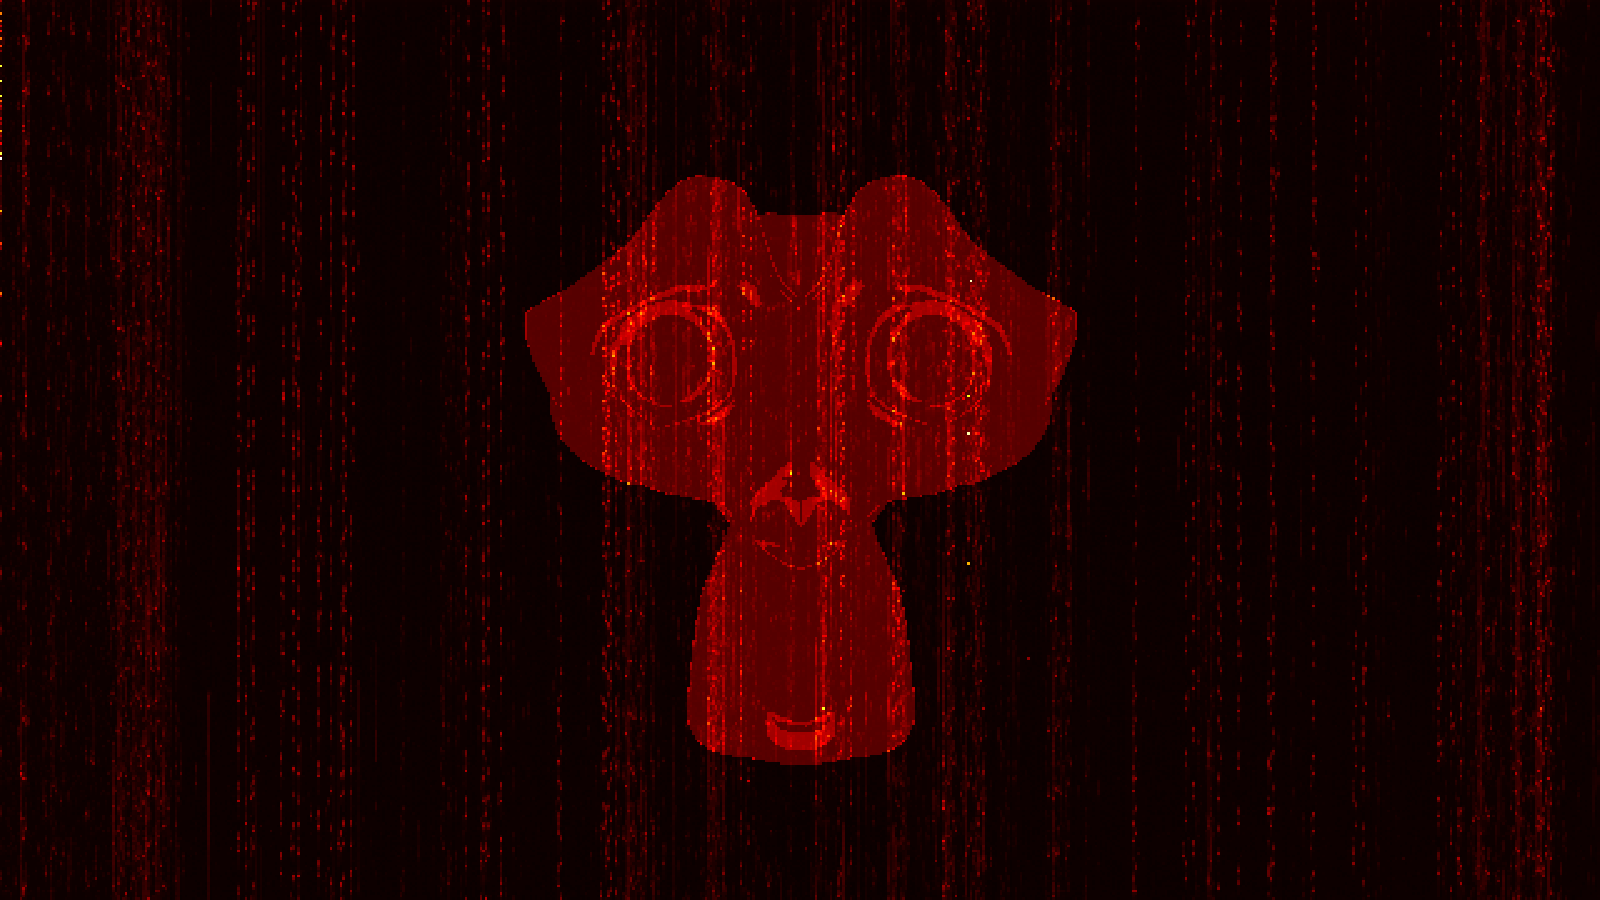
\includegraphics[width=15cm]{normal.png}
\end{figure}

Na powyższej mapie cieplnej widzimy, że najwięcej czasu algorytm spędził na generowaniu pikseli zawierających model.

\begin{figure}[h!]
\centering
  \caption{Brak wykorzystanie bryły otaczającej}
  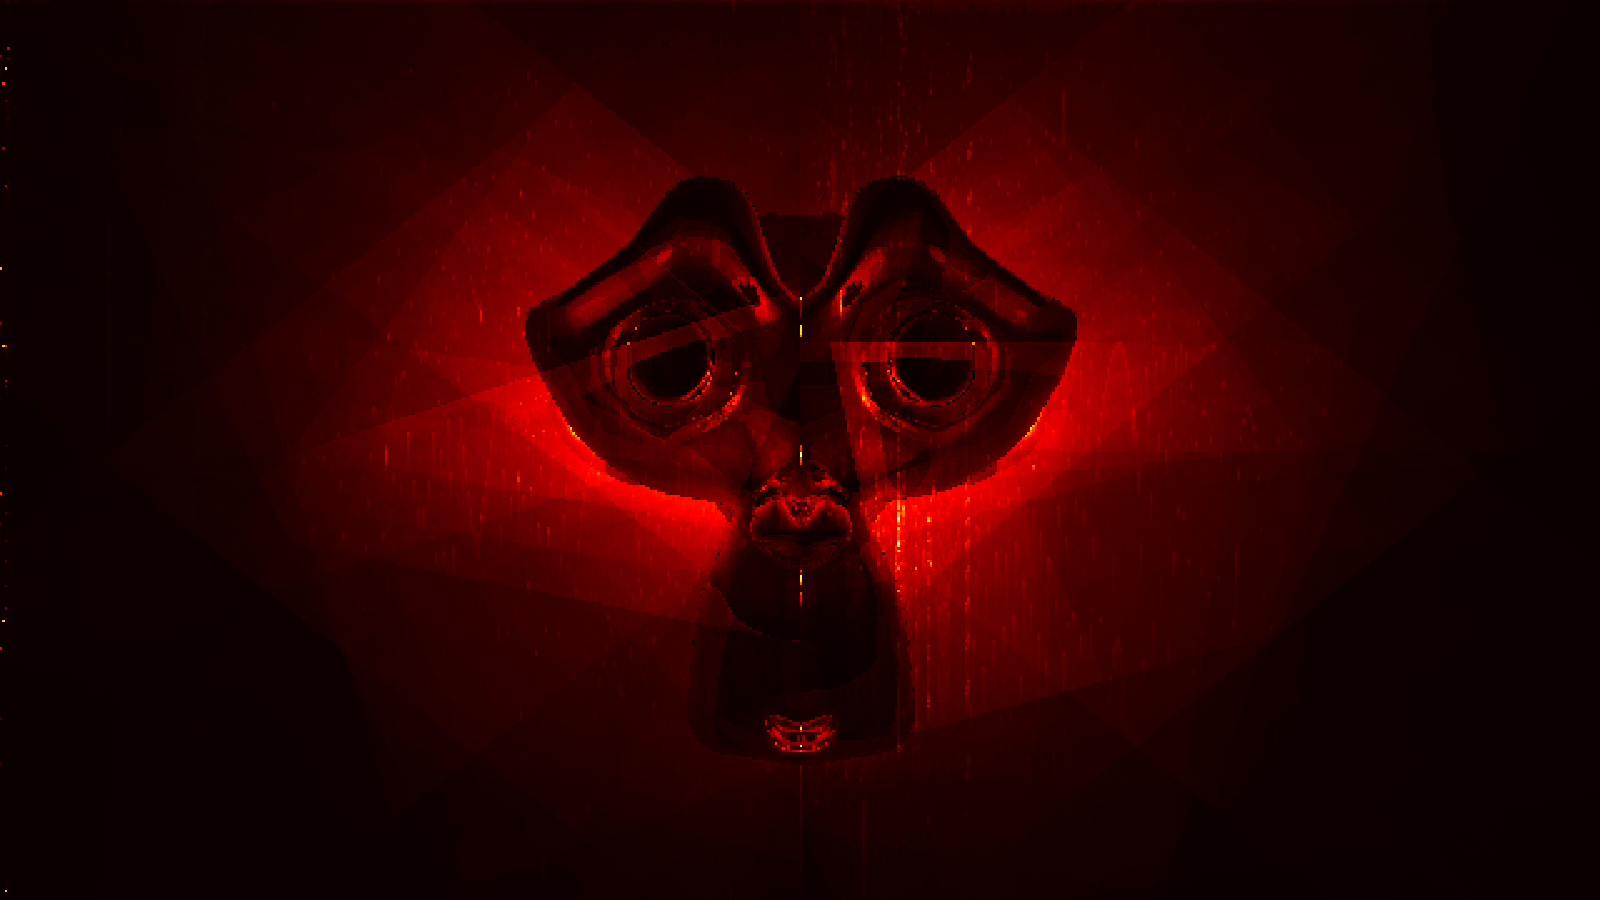
\includegraphics[width=15cm]{noaabb.png}
\end{figure}

W przypadku zastosowania drzewa BSP ciężar obliczeń spadł na otoczenie modelu a nie na sam model. Powyższy obraz w interesujący sposób przedstawia płaszczyzny dzielące przestrzeń. Elementy znajdujące się za większą liczbą płaszczyzn są jaśniejsze. 

\begin{figure}[h!]
\centering
  \caption{Z wykorzystaniem bryły otaczającej}
  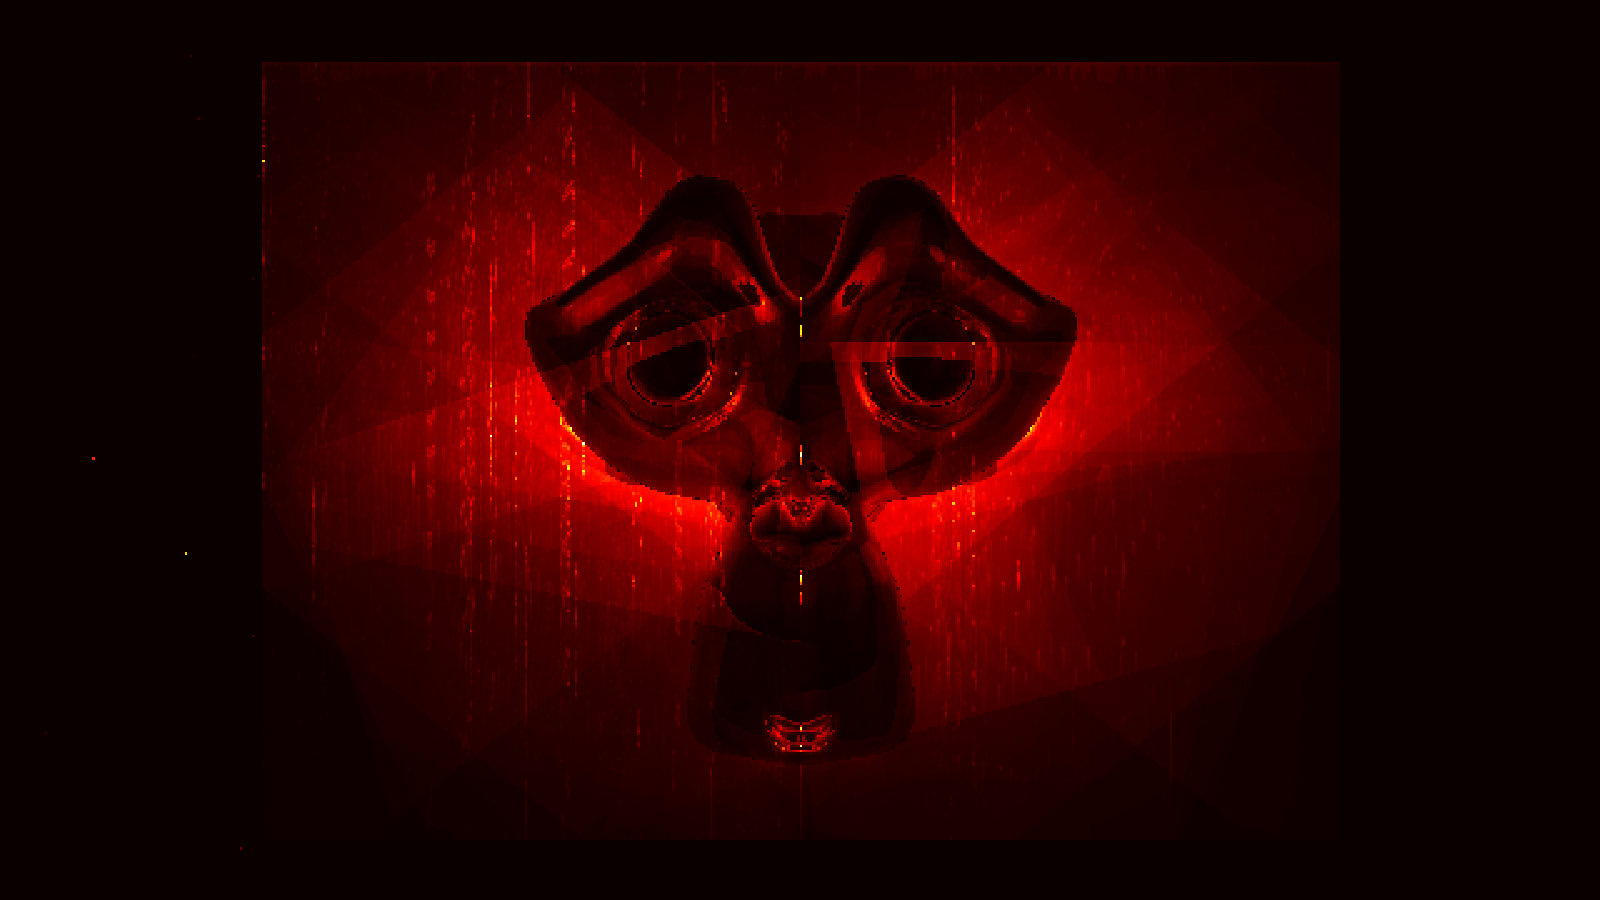
\includegraphics[width=15cm]{aabb.png}
\end{figure}

Zastosowanie bryły otaczającej sprawia, że czas liczenia promieni nie trafiających w żaden obiekt maleje właściwie do zera (koszt badania przecięcia promienia z bryłą otaczającą). Wbrew temu, co może sugerować powyższy obraz, każda ze ścian bryły otaczającej jest styczna do modelu - wrażenie, że jest inaczej powoduje rzut perspektywiczny (elementy, które są bliżej nas, zdają się być większe). Nie byłoby, tak gdyby został zastosowany rzut prosty.

Na podstawie powyższych informacji można wywnioskować, że zastosowanie brył otaczających, które lepiej przylegałyby do modeli, zmniejszy czas wykonywania obliczeń. Dodatkowo, chcąc wprowadzić funkcję SAH niezbędne, jest zamknięcie całej sceny w bryle, ponieważ ta wymaga liczenia objętości podprzestrzeni (musi więc istnieć jakieś ograniczenie). Naturalnym rozwinięciem wydaje się również wprowadzenie hierarchii brył otaczających - na podstawie powyższej analizy zdaje się, że każdy integralny i nieruchomy obiekt powinien być najpierw zamknięty w bryle, a następnie dzielony z wykorzystaniem drzewa BSP. Rozwiązania hybrydowe są szeroko stosowane w grafice, zwłaszcza, że drzewo BVH ma tą wyższość nad drzewem BSP, że przemieszczanie się obiektów nie wymaga przebudowania go całego.

\section{Przykładowe obrazy}


\begin{figure}[htb!]
\centering
  \caption{Spheres}
  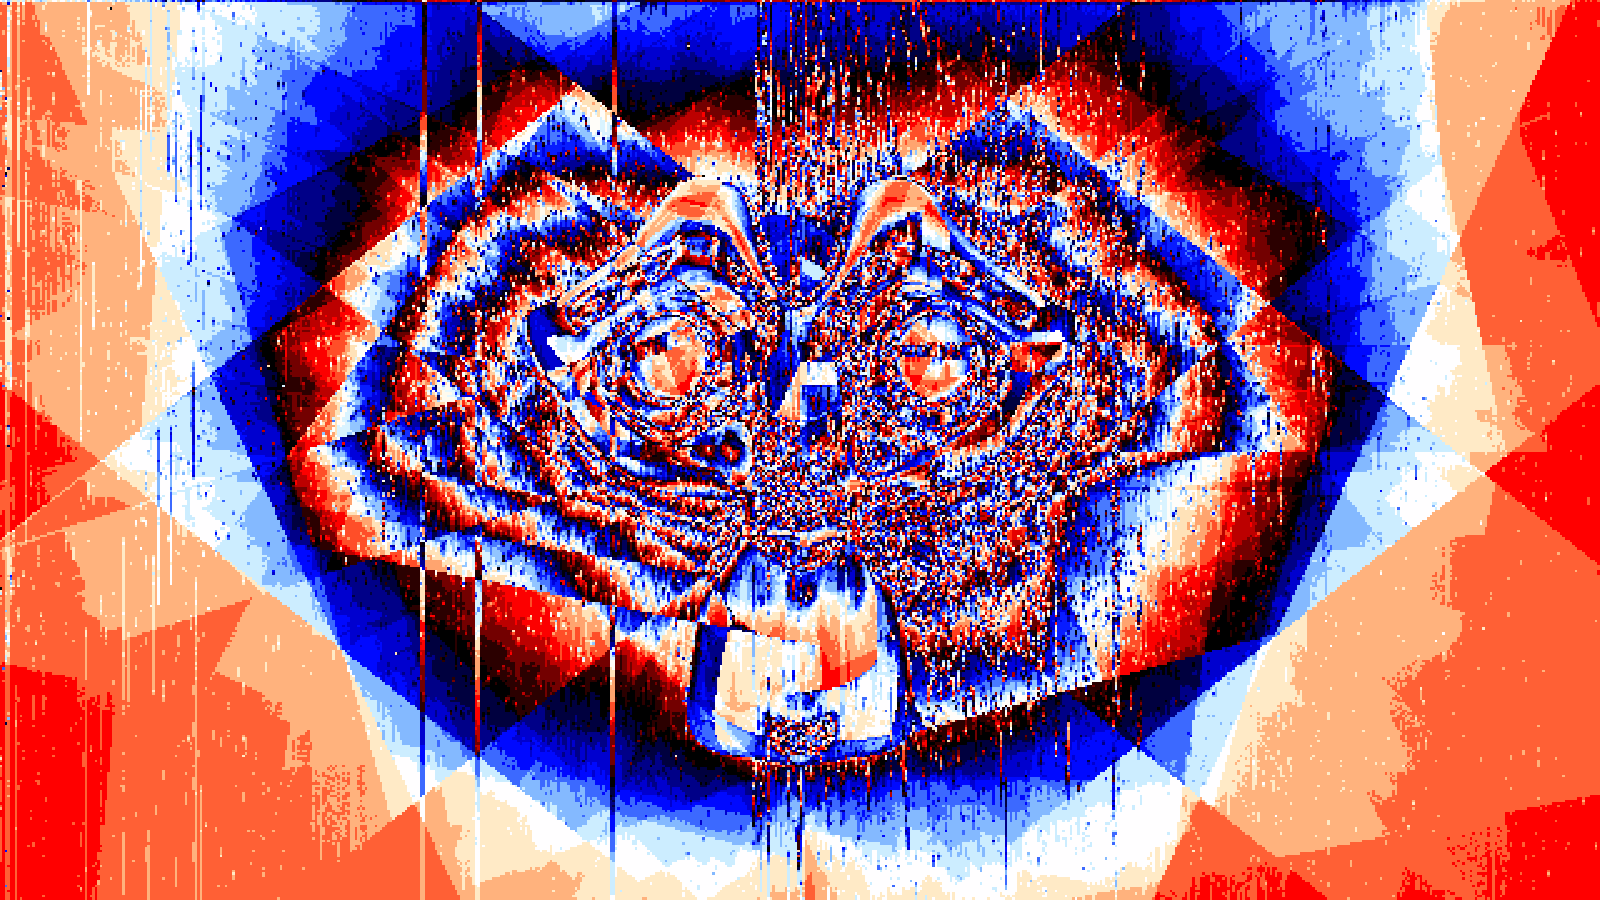
\includegraphics[width=\textwidth]{psycho.png}
\end{figure}


\begin{figure}[htb!]
\centering
  \caption{Spheres}
  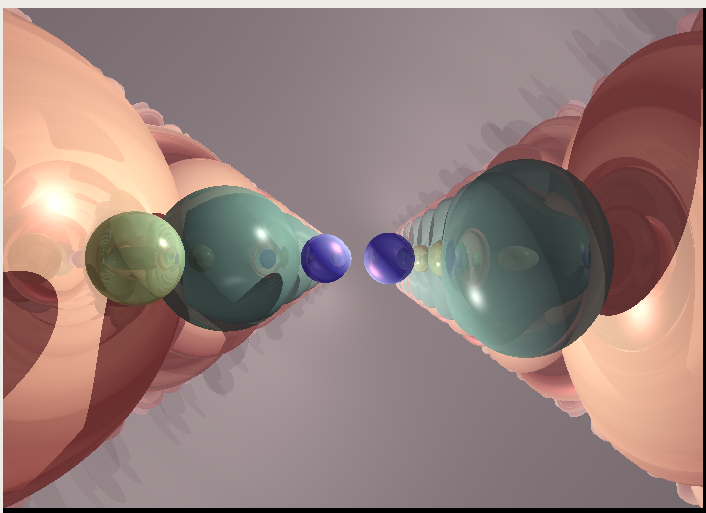
\includegraphics[width=\textwidth]{mirror.png}
\end{figure}


\begin{figure}[htb!]
\centering
  \caption{Spheres}
  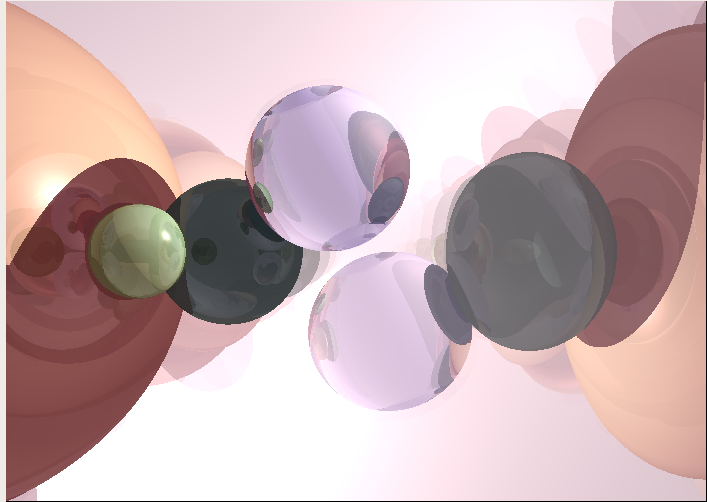
\includegraphics[width=\textwidth]{glasssphere.png}
\end{figure}

\begin{figure}[htb!]
\centering
  \caption{Spheres}
  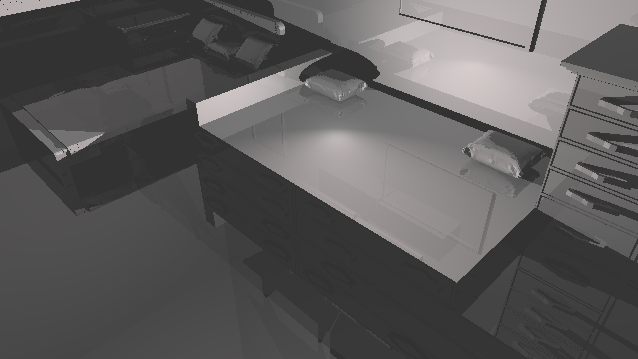
\includegraphics[width=\textwidth]{light8s.png}
\end{figure}


\begin{figure}[htb!]
\centering
  \caption{Spheres}
  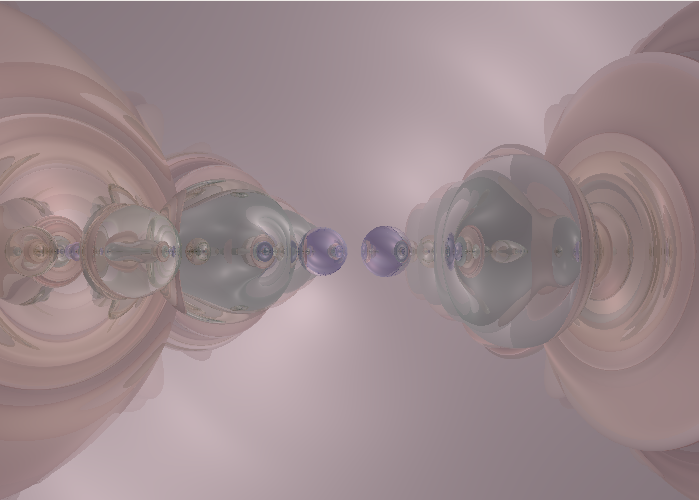
\includegraphics[width=\textwidth]{water.png}
\end{figure}

\begin{figure}[htb!]
\centering
  \caption{Spheres}
  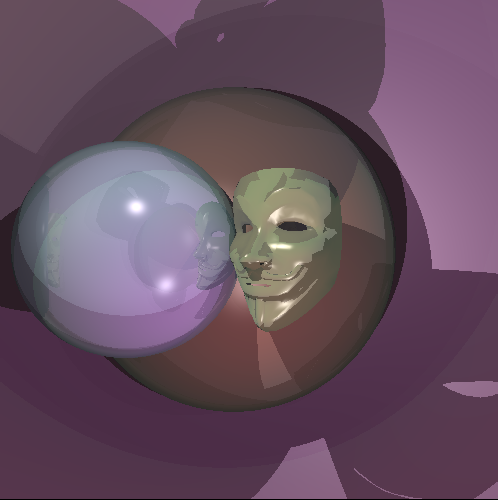
\includegraphics[width=\textwidth]{mask.png}
\end{figure}

